\section{Exploratory Model Evaluation and Linguistic Validation}
\label{sec:pilot}

This section reports the genuine model outcomes obtained under the framework and their linguistic
validation, in chronological order: two complete registered pilot runs of 1,512 calls each, executed on
27 October 2026 on the pilot split (the first six subsections below); a supplemental quantized evaluation
of four open-weight scales over 16,618 matched prompts each (Section~\ref{sec:p1-local}); and the
subsequently completed two-reviewer Turkish linguistic review of 360 stimuli sampled from the same frozen
prompt population (Section~\ref{sec:review}). Every model result in this section is \emph{exploratory}: the
runs exercise the full execution and analysis machinery and motivate the confirmatory design, but the
execution-gate receipts for confirmatory authorization were not issued, no frozen-test evaluation has been
performed, and RQ1--RQ5 are not answered confirmatorily.

\subsection{Runs, shared cohort, and execution integrity}

Two registered model configurations were enabled by explicit user selection: Qwen2.5-0.5B-Instruct at a
pinned immutable revision, executed locally with greedy decoding (CPU, float32), and the dated snapshot
\texttt{gpt-4o-2024-08-06}, queried through its provider API at temperature zero. Both runs executed the
same immutable plan cohort: entity counts $n \in \{4, 8, 16, 32\}$ with eight latent orders per size,
endpoint, internal, and distance-controlled queries, the \texttt{spatial\_front} relation,
\texttt{native\_shared} names, English canonical and equivalent conditions, and all seven Turkish
conditions (canonical, general equivalent, and P1--P5). Each of the nine language/presentation conditions
contains the same 168 planned queries; prompts are byte-identical across models.

\begin{table}[t]
  \centering
  \caption{Executed pilot runs. Both runs completed all planned calls with zero invalid and zero
  wrong-language answers under the strict parser.}
  \label{tab:pilotruns}
  \small
  \begin{tabular}{@{}llrr@{}}
    \toprule
    Model & Execution & Calls & Invalid \\
    \midrule
    Qwen2.5-0.5B-Instruct & local, greedy, CPU/float32 & 1\,512/1\,512 & 0 \\
    gpt-4o-2024-08-06     & provider API, temperature 0 & 1\,512/1\,512 & 0 \\
    \bottomrule
  \end{tabular}
\end{table}

Execution followed the audited protocol without exception: write-once plans re-derived and byte-compared
at execution time, append-only raw request/response records with full lineage, and checkpointed resumption.
One transient transport error occurred in the API run; following the ambiguity policy, the run halted and
resumed only after an explicit, logged retry resolution acknowledging duplicate risk. Two earlier API run
identifiers are retained as provenance of failed attempts (a local TLS misconfiguration before any billable
call, and a provider spending-limit refusal with zero billed generations); neither contributes records to
the analyzed run.

\subsection{A degenerate responder: perfect invariance without competence}

Qwen2.5-0.5B-Instruct emitted a constant answer per language on all 1,512 prompts: affirmative
(\emph{YES}) on every English prompt and negative (\emph{HAYIR}) on every Turkish prompt, at every size,
query type, and presentation. Because planned gold labels are balanced, marginal accuracy is exactly 0.500
in every stratum and the paired Turkish--English difference is zero everywhere. Raw invariance is perfect:
$\widehat{I} = 1$ within each language, with $\widehat{R} = \widehat{D} = 0.5$ and $\widehat{U} = 0$.
The pooled answer rate is degenerate ($q \in \{0, 1\}$), so $I_e = 1$ and $\kappa_{\mathrm{CBE}}$ is
undefined with the recorded reason \texttt{constant\_pooled\_answer}, exactly as
Equation~\eqref{eq:kappa} prescribes.

This run is a concrete demonstration of the framework's central measurement argument rather than a mere
null result. An evaluation reporting raw cross-presentation agreement would have scored this model as
perfectly robust; the joint presentation of $R$, $D$, $U$, and the chance correction instead identifies a
responder whose ``consistency'' consists entirely of shared correct-by-chance and shared wrong answers.
No competence claim, positive or negative, beyond this behavioral characterization is made for the model.

\subsection{GPT-4o: graded competence and a presentation cliff}

All 1,512 GPT-4o answers were valid and in the requested language, so all-planned and valid-pair
denominators coincide and valid-pair coverage is 1 in every stratum below. Figure~\ref{fig:pilot}
summarizes the marginal structure. Pooled all-planned accuracy is 72.0\% on English ($N = 336$) and
57.8\% on Turkish ($N = 1{,}176$). The two English conditions agree closely (canonical 71.4\%, equivalent
72.6\%), while the Turkish conditions separate: canonical 67.9\% and P1 68.5\% at the top; equivalent
57.7\%, P2 58.3\%, P4 61.9\%, and P5 53.6\% in between; and P3, the alternative constituent construction,
at 36.9\% --- below the 50\% balanced baseline.

\begin{figure}[t]
  \centering
  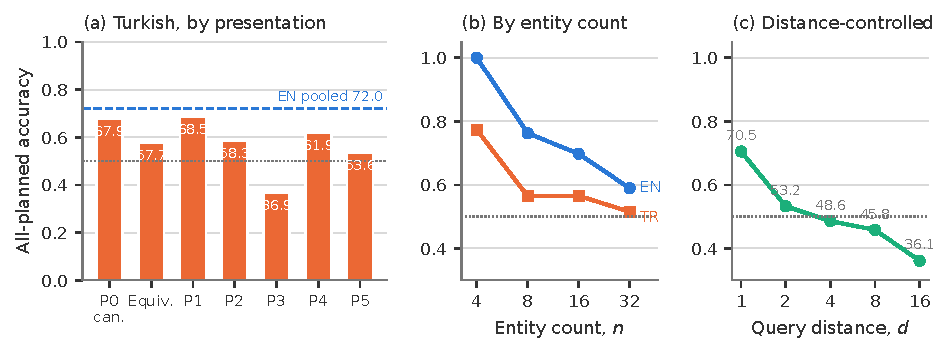
\includegraphics[width=\linewidth]{figures/manuscript/fig5_pilot_gpt4o.pdf}
  \caption{Exploratory pilot accuracy of \texttt{gpt-4o-2024-08-06} (all answers valid; all-planned
  accuracy; dotted line: 50\% balanced baseline). (a) Turkish accuracy by presentation condition with the
  pooled English reference; 168 prompts per condition. (b) Accuracy by entity count and language.
  (c) Pooled accuracy of distance-controlled queries by latent query distance $d$; per-distance counts
  vary by design (288, 216, 216, 144, and 72 prompts). Pilot split, one relation family, stimulus review
  in Section~\ref{sec:review}; these curves are not confirmatory answers to RQ1--RQ3.}
  \label{fig:pilot}
\end{figure}

Accuracy declines monotonically with entity count in both languages (English $100\% \to 58.9\%$ and
Turkish $77.4\% \to 51.5\%$ from $n = 4$ to $n = 32$) and with latent query distance within the
distance-controlled stratum ($70.5\%$ at $d = 1$ to $36.1\%$ at $d = 16$). The pooled query-type ordering
is endpoint $76.4\%$ $>$ internal $64.9\%$ $>$ distance-controlled $55.0\%$. Sustained below-baseline
accuracy at large $d$ indicates a systematic directional error rather than random guessing. Predicted
answer rates also differ by language: the affirmative rate is 0.476 on English but 0.680 on Turkish
against balanced gold labels, i.e.\ Turkish errors skew toward \emph{EVET}.

\begin{table}[t]
  \centering
  \caption{Pooled descriptive paired profiles for GPT-4o (168 jointly valid pairs per row; valid-pair
  coverage 1.0, so Equations~\eqref{eq:identities}--\eqref{eq:strict} coincide with their all-planned
  counterparts). $q$ is the pooled affirmative rate of Equation~\eqref{eq:kappa}. Pooling crosses size and
  query-type strata, so these values are summaries of the executed cohort, not stratum estimands;
  per-stratum profiles with cluster-bootstrap intervals are in the released analysis tables.}
  \label{tab:pilotprofiles}
  \small
  \begin{tabular}{@{}lccccc@{}}
    \toprule
    Comparison & $R$ & $D$ & $U$ & $q$ & $\kappa_{\mathrm{CBE}}$ \\
    \midrule
    TR canonical $\to$ TR equivalent & 0.458 & 0.202 & 0.339 & 0.652 & 0.253 \\
    TR canonical $\to$ TR P1         & 0.565 & 0.202 & 0.232 & 0.640 & 0.496 \\
    TR canonical $\to$ TR P2         & 0.500 & 0.238 & 0.262 & 0.667 & 0.411 \\
    TR canonical $\to$ TR P3         & 0.298 & 0.250 & 0.452 & 0.673 & $-0.027$ \\
    TR canonical $\to$ TR P4         & 0.542 & 0.244 & 0.214 & 0.631 & 0.540 \\
    TR canonical $\to$ TR P5         & 0.446 & 0.232 & 0.321 & 0.667 & 0.277 \\
    EN canonical $\to$ TR canonical  & 0.565 & 0.173 & 0.262 & 0.560 & 0.469 \\
    EN equivalent $\to$ TR equivalent & 0.476 & 0.173 & 0.351 & 0.568 & 0.284 \\
    \bottomrule
  \end{tabular}
\end{table}

Table~\ref{tab:pilotprofiles} gives the pooled paired decomposition. The P3 contrast is qualitatively
different from every other Turkish perturbation: robust correctness falls to $\widehat{R} = 0.298$,
presentation dependence rises to $\widehat{U} = 0.452$, and the pooled chance-corrected agreement is
approximately zero ($\kappa_{\mathrm{CBE}} = -0.027$) --- the model's answers under the canonical and P3
realizations of the same latent query are statistically unrelated. The cross-language rows show the second
mechanism the decomposition separates: moving from English to Turkish converts correct answers into
presentation-dependent ones ($U$ up to 0.351) rather than into shared errors ($D$ stable at 0.173).

\subsection{Inferential results at pilot power}

Declared-family inference behaves as the design anticipates at this scale. Across the 70 matched
Turkish--English strata, the accuracy difference is negative in 31 and positive in 10 (mean $-0.098$), but
no individual eight-pair stratum survives Holm correction: the direction is consistent while per-stratum
McNemar tests are underpowered, which is precisely the regime the frozen-test sample sizes were chosen to
escape. The P3 effect, by contrast, is strong enough to register even here: the canonical-versus-P3
family contains the only Holm-surviving strata in the study (two strata at $n = 32$, endpoint and
distance-controlled, each with difference $-0.75$ and Holm-adjusted $p = 0.031$). Cluster-bootstrap
intervals accompany every reported stratum in the released tables; pooled values above are descriptive.

\subsection{Exploratory lexical-direction diagnostics (RQ4)}

The retained lexical pipeline was additionally executed joined to both completed runs, producing the
declared answer-share diagnostics, lexical-direction profiles, Spearman associations, and controlled
regression specifications on the pilot observations. Its most interpretable output is a pronounced
\emph{direction asymmetry} in GPT-4o (Table~\ref{tab:direction}): against balanced gold labels, queries
asked with the inverse predicate (Turkish \emph{arkasındadır}, English \emph{behind}) are answered
affirmatively far more often and less accurately than forward queries (\emph{önündedir} / \emph{in front
of}). The asymmetry appears in both languages and is largest in Turkish, where the inverse-direction
affirmative share reaches 0.793; it accounts for most of the pooled Turkish affirmative bias reported
above. The predeclared response-tendency diagnostic flags Qwen2.5-0.5B in every stratum (excessive
\emph{no} in Turkish, excessive \emph{yes} in English), while GPT-4o pools within thresholds overall and
crosses the affirmative threshold only in inverse-direction Turkish strata.

\begin{table}[t]
  \centering
  \caption{Direction-specific pilot diagnostics for GPT-4o (all planned gold labels balanced at 0.500;
  all answers valid). Forward queries use \emph{önündedir} / \emph{in front of}; inverse queries use
  \emph{arkasındadır} / \emph{behind}. These are descriptive shares on one relation family; direction
  changes the lexical predicate, the construction, and tokenization together, so no single cause is
  identified.}
  \label{tab:direction}
  \small
  \begin{tabular}{@{}llrcc@{}}
    \toprule
    Language & Query direction & $N$ & Accuracy & Affirmative share \\
    \midrule
    Turkish & forward & 588 & 0.639 & 0.568 \\
    Turkish & inverse & 588 & 0.517 & 0.793 \\
    English & forward & 168 & 0.768 & 0.399 \\
    English & inverse & 168 & 0.673 & 0.554 \\
    \bottomrule
  \end{tabular}
\end{table}

This asymmetry aligns suggestively with the preprocessing measurements: the forward lemma \emph{ön} is
more than twice as frequent as the inverse lemma \emph{arka} in the retained corpus measurement
(Table~\ref{tab:lemma}), and for the GPT-4o encoding the inverse Turkish predicate is four times its
English counterpart's token length while the forward pair is matched (Figure~\ref{fig:tokens}). The
design, however, cannot promote this alignment to an association: the pilot cohort contains a single
relation family, so each correlation cell holds at most two lexical units, and the retained Spearman and
regression outputs record exactly that --- the large majority of cells return \texttt{constant\_input},
\texttt{insufficient\_pairs}, \texttt{insufficient\_rows}, or \texttt{rank\_deficient} rather than a
coefficient, as the protocol requires of unsupported or collinear fits. RQ4's association component
therefore remains unanswered; answering it requires the multi-relation frozen design, where the nine
relation families provide the cross-vocabulary variation this cohort lacks.

\subsection{Training backend execution (RQ5)}

The optional adaptation backend was executed for the first time on rented CUDA hardware (RTX 6000 Ada,
48\,GB, bf16) under the configuration's declared dependency pins, which this run validates. All five
training arms of the pilot profile --- LoRA SFT, paired SFT, SFT with the JS consistency term, and both
GRPO objectives --- completed on Qwen2.5-1.5B-Instruct from a hash-verified local weights bundle, with
immutable plans, zero gate blockers, recorded hardware and token budgets, and deterministic seeding. The
pilot profile is smoke-scale by design (two optimizer steps per arm), so these runs validate the training
machinery and its accounting, not any adaptation effect. Both GRPO arms recorded one zero-gradient step,
the exact diagnostic the plan's warnings predict for binary prompt-normalized advantages. The matched
base-versus-adapter evaluation remains unexecuted: the protocol's evaluation design is frozen at nine
sizes on the test split (10,224 calls per arm), which requires a dataset-bound execution-gate review
receipt that has not been issued (the completed stimulus review of Section~\ref{sec:review} is a separate
instrument); no reduced evaluation is expressible within the validated configuration, deliberately. RQ5
therefore remains empirically unanswered, with trained adapters retained should that receipt be produced.

\subsection{Supplemental quantized local evaluation: an open-weights scale sweep}
\label{sec:p1-local}

To test whether the pilot's findings are idiosyncrasies of one proprietary model, the frozen protocol was
additionally executed across the Qwen2.5 instruction-tuned family at four scales (0.5B, 3B, 7B, 14B) in a
\emph{supplemental quantized local arm}: Q4\_K\_M GGUF weights served by Ollama (weight digests recorded
per run), greedy decoding at temperature 0 with fixed seed, the audited message constructor with run-time
prompt-hash re-verification, and the registered strict parser. Because quantized weights are not the
registered fp/bf16 snapshots, this arm is labeled on every record and is never pooled with
registered-provider results; agreement across arms is read as qualitative replication, not equivalence.
The expanded manifest holds 16{,}618 prompt identities drawn exclusively from the pilot split (all nine
relation families, sizes $4 \le n \le 128$, balanced paired sampling across languages, presentations, and
naming controls; the frozen test sizes remain untouched), and every prompt passed an automated semantic
validation of its stated facts and gold label before execution. All four arms answered all 16{,}618
prompts with zero transport failures; unparseable responses (0, 25, 184, and 247 from 0.5B to 14B, the
latter coinciding with output-length truncation) are retained and scored as errors under the all-planned
estimand. Like the pilot, this expanded run exceeds the predeclared human-review threshold; the stimulus
review of Section~\ref{sec:review} was subsequently completed on this run's prompt population, but no
execution-gate receipt was issued, and the arm remains exploratory (quantized weights, pilot split).

\begin{figure}[t]
  \centering
  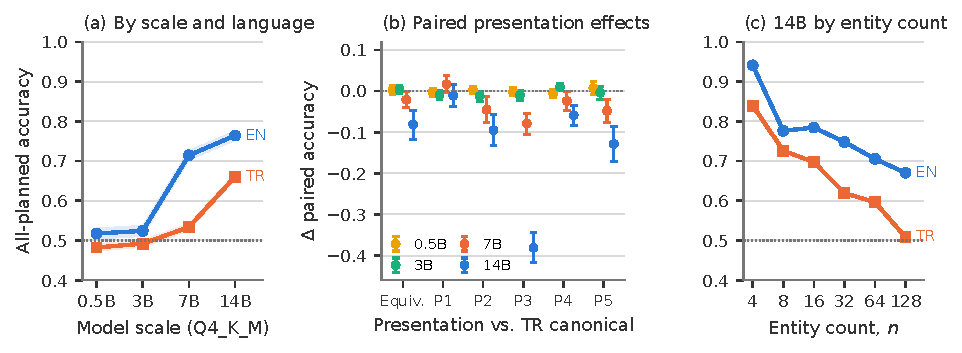
\includegraphics[width=\linewidth]{figures/manuscript/fig6_p1_quantized_scaling.pdf}
  \caption{Supplemental quantized local evaluation of the Qwen2.5 instruct family (Q4\_K\_M; all-planned
  accuracy over 16{,}618 prompts per model; dotted lines: 50\% balanced baseline and zero effect).
  (a) Accuracy by model scale and language with Wilson bands. (b) Query-matched paired accuracy change of
  each Turkish presentation against the Turkish canonical form, with latent-cluster bootstrap 95\%
  intervals; pooled single-condition accuracies are compositionally confounded and are not shown.
  (c) Accuracy by entity count for the 14B model. Pilot split, quantized supplemental arm, stimulus
  review in Section~\ref{sec:review}; not confirmatory answers to RQ1--RQ3.}
  \label{fig:p1scaling}
\end{figure}

The sweep reproduces both pilot regimes and locates the transition between them
(Figure~\ref{fig:p1scaling}a). The 0.5B and 3B models are near-constant responders --- 0.5B answers
\emph{hay\i{}r} on 95.8\% of Turkish and \emph{yes} on 99.8\% of English calls, and its paired
English--Turkish profile is the degenerate signature in pure form ($R = 0.017$, $U = 0.970$: on almost
every matched pair exactly one language is ``correct'' because the two constant answers disagree).
Discrimination emerges at 7B in English only (71.4\% vs.\ 53.4\%; paired gap $-0.176$, cluster-bootstrap
95\% CI $[-0.241, -0.106]$) and reaches both languages at 14B (76.4\% vs.\ 66.1\%; paired gap $-0.075$,
CI $[-0.126, -0.020]$). Because pooled pairs share latent orders, ordinary McNemar inference is undefined
for these contrasts; all language and presentation intervals are latent-cluster bootstrap contrasts and
are labeled exploratory.

Two pilot findings replicate in open weights and sharpen with scale. First, the P3 presentation cliff:
query-matched P3 costs the 14B model $38.1$ points of paired accuracy against the Turkish canonical form
(CI $[-0.418, -0.344]$; 554 vs.\ 40 discordant pairs), dropping P3 accuracy to 43.1\% --- below the
balanced baseline --- while the same contrast at 7B is already credible at $-7.9$ points and absent in the
constant responders (Figure~\ref{fig:p1scaling}b). Per-stratum agreement decays with complexity
($\kappa_{\mathrm{CBE}}$ for canonical-versus-equivalent at 14B: $0.57$ at $n{=}4$ to $0.12$ at
$n{=}128$), and for canonical-versus-P3 it turns negative at $n{=}16$ and $n{=}32$: systematic answer
flips, not noise. Second, the complexity decay: 14B Turkish accuracy falls monotonically from 83.9\% at
$n{=}4$ to 50.8\% --- chance --- at $n{=}128$ (English 94.1\% to 67.0\%; Figure~\ref{fig:p1scaling}c),
mirroring the GPT-4o pilot curve. The naming family, whose pairs are cluster-unique and therefore admit
exact inference, adds one Holm-surviving result: at 14B, replacing native Turkish entity names with shared
symbolic labels costs $11.7$ points (McNemar $b{=}59$, $c{=}24$, Holm-adjusted $p = 3.8\times10^{-4}$),
while English transliteration of the same names costs nothing measurable --- once competence exists,
entity-name surface form matters, and the deficit is not explained by transliteration alone.

\subsection{Completed two-reviewer Turkish linguistic review}
\label{sec:review}

The human review that the construction audit required was executed by two independent Turkish-proficient
reviewers on a 360-item stratified sample drawn from the frozen pilot-split prompts (all nine relation
families, every Turkish presentation, P3 deliberately oversampled at 144 items; annotation protocol,
blinding, and the inclusion policy were fixed before any judgment was entered). Each reviewer
independently rated grammaticality and naturalness (1--5), semantic equivalence of each transformed
prompt against its canonical counterpart, and clause-level ambiguity. The predeclared policy admits a
transformed item to confirmatory analysis only when both reviewers rate grammaticality $\ge 4$ and agree
the transformation is meaning-preserving.

The outcome is sharply structured. Semantic equivalence is unanimous: both reviewers judged all 324
transformed items meaning-preserving, and no item was flagged ambiguous. Grammaticality excluded exactly
one construction: the P3 realization of \emph{temporal\_completion}, whose 16 sampled items one reviewer
rated ungrammatical (grammaticality 2, ``devrik c\"umle yap\i{}s\i{}''), leaving 344 of 360 items
confirmatory-eligible. Naturalness --- which the policy deliberately records but does not gate on --- is
the one contested dimension: exact inter-reviewer agreement is low (33\%, Cohen's $\kappa = 0.06$), the
two reviewers' P3 naturalness medians are 4 versus 2, and only 6 of 144 P3 items received $\ge 4$ from
both. (Chance-corrected agreement is degenerate for grammaticality and ambiguity because one or both
reviewers used a single category almost everywhere; raw agreement is 96\% and 100\%.)

The review therefore narrows, but does not fully close, the stimulus-artifact explanation of the P3
cliff. A review-driven sensitivity reanalysis removes the excluded relation entirely from the P3
contrast: the 14B query-matched deficit survives unchanged or deepens ($-0.381$ over all nine relations
versus $-0.408$, cluster-bootstrap 95\% CI $[-0.446, -0.370]$, with \emph{temporal\_completion} removed;
the 7B contrast is unchanged at $-0.080$). The P3 collapse is thus measured on stimuli that two
independent reviewers unanimously certify as meaning-preserving and (outside one excluded construction)
grammatical, while their discourse naturalness remains contested --- the honest residual reading is that
models fail on grammatical, truth-preserving but discourse-atypical constituent orders, a regime in which
a competent human reader does not lose the ability to evaluate the stated facts. Review artifacts,
per-item decisions, and agreement statistics are released with the framework
(\texttt{validation/review\_results/}); the separate execution-gate receipts for runs above the declared
call threshold were not issued, so no evaluation in this manuscript claims confirmatory status.

\subsection{What this evaluation does and does not establish}

These experiments establish that the end-to-end protocol --- immutable planning, gated execution, strict
parsing, paired analysis with declared denominators, and multiplicity control --- runs unmodified on local,
provider-hosted, and quantized local models, and that the paired decomposition discriminates in practice
between degenerate constant responders and models with graded, presentation-sensitive competence, with the
same qualitative structure recurring from the registered pilot to the digest-pinned nine-relation sweep.
They do not establish a confirmed Turkish--English gap, a morphology effect, or a complexity law:
everything remains on the pilot split; strata share latent orders; and the supplemental arm is quantized
and therefore not precision-comparable to registered snapshots. Section~\ref{sec:discussion} synthesizes
the findings and their interpretive boundaries, including what the completed review does and does not
resolve about P3. These results size and motivate, but do not replace, the preregistered frozen-test
evaluation.
